\section{Simple mathematical computation example for Parallel Programming} \label{chap:simpleMathCompParallel}

Before going into detail about the Mandelbrot computation, we will discuss as a first example a basic computation as already mentioned in Chapter \ref{chap:mathComp}. The reason we are doing that is to reduce complexity and to point out the main parts, we will need for the Mandelbrot computation as well. In formula \ref{formula:scalarProdSeq}, we have pointed out that the computation of a simple scalar product of two vectors with the same dimension \textit{N} can be split into several sub task \textit{p}. Our modified version is based on two sums. The outer one will iterate [index \textit{i}, see formula \ref{formula:twoLoopSum}] from zero to an upper limit \textit{N\textsubscript{1}} and sum up the result from the inner sum, which will perform a sum from 0 to \textit{N\textsubscript{2}} [index \textit{j}, see formula \ref{formula:twoLoopSum}] over a multiplication of \textit{i} and \textit{j}. The following formula represent the announced mathematical problem:

\begin{align} \label{formula:twoLoopSum}
\begin{aligned}
s &= \sum_{i = 0}^{N_1} \left( \sum_{j = 0}^{N_2} \left(i \cdot j\right) \right)
\end{aligned}
\end{align}
\

To process the problem in parallel, it is only possible to seperate the outer sum into sub sums regarding to formula \ref{formula:twoLoopSumParallel}.

\begin{align} \label{formula:twoLoopSumParallel}
\begin{aligned}
s &= \sum_{i = 0}^{N_1} \left( \sum_{j = 0}^{N_2} \left(i \cdot j\right) \right)
\\ &=  \underbrace{ 
	\sum_{i = 0}^{\frac{N_1}{2} - 1} \left( \sum_{j = 0}^{N_2} \left(i \cdot j\right) \right)
}_\text{p\textsubscript{0}} \qquad \vertarrowbox{+}{process communication} \qquad \underbrace{  
	\sum_{i = \frac{N_1}{2}}^{N_1} \left( \sum_{j = 0}^{N_2} \left(i \cdot j\right) \right)
}_\text{p\textsubscript{1}}
\end{aligned}
\end{align}
\

For collecting the part results from the parallel computed sums, some sort of process communication [see formula \ref{formula:twoLoopSumParallel}] between the threads is necessary, more then, its impossible without it. 

\newpage

But actually, this is the task, we have to take care about most. Otherwise we will run into race conditions while addressing same resources or even blocking methods, which will result in wrong execution time measurements.

As mentioned in Chapter \ref{chap:parPrgModels}, a common solution to communicate between threads running on different cores is using the \textbf{Message Passing Model} [for more details, see Chapter \ref{subsection:processInteraction}]. Our aim is to pass the computed part results to a main ``actor'', which will collect the part sums to calculate the final result. Furthermore, for bench-marking this setup, we will implement a time measurement mechanism to evaluate the decrease of execution time running the computation on one or both cores. 

Formula \ref{formula:twoLoopSumParallel} is theoretically not limited to the dedicated number of cores, which the hardware platform offers. Each core can handle multiple threads, but in this case, we would leave real time parallelism, because each core now has to handle multiple threads by the scheduler. Every thread on each core will be given some execution time between switching the context to the next one. An overall speedup is not guaranteed with this method.   

\newpage

\subsection{UML diagram}

This little mathematical example can be found on our GitHub repository \parencite{internet12} and is basically split into three parts. The main \textit{*.ino} file, and two classes, the \textit{Computation.h} and the \textit{Benchmark.h}. 

\begin{figure}[htbp]
	\centering
	\begin{subfigure}{.5\textwidth}
		\centerline{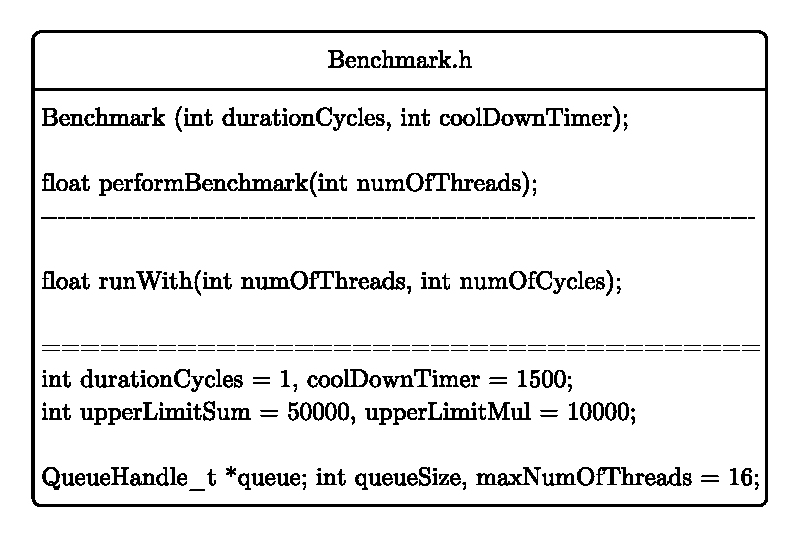
\includegraphics[width=1\linewidth]{images/Benchmark-UML.pdf}}
		\caption{ UML diagram Benchmark.h class }
		\label{fig:benchUML}
	\end{subfigure}%
	\begin{subfigure}{.5\textwidth}
		\centerline{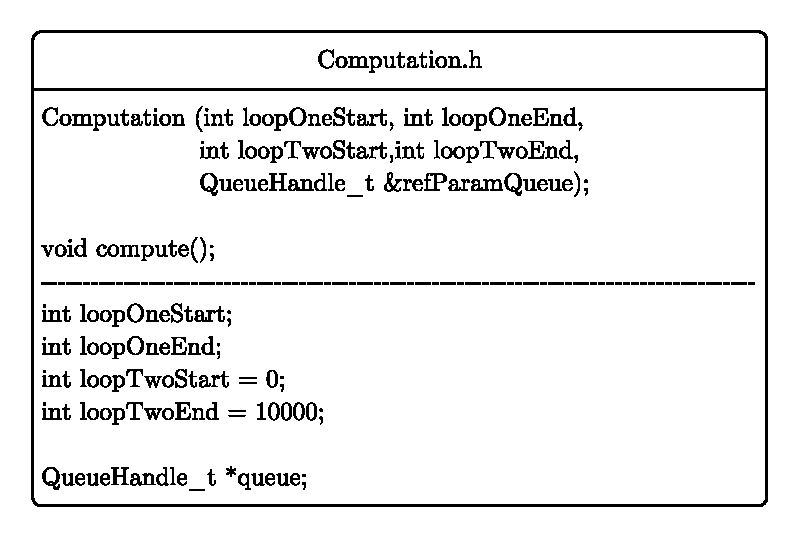
\includegraphics[width=1\linewidth]{images/Computation-UML.pdf}}
		\caption{ UML diagram Computation.h class }
		\label{fig:compUML}
	\end{subfigure}
	\caption{Overview over both main implementations regarding Chapter \ref{chap:simpleMathCompParallel}}
	\label{fig:umlDiagrBasicExample}
\end{figure}

\subsection{Implementation}

The \textit{Benchmark.h} class has several functions to set the necessary parameters to start a benchmark like mentioned at the end of Chapter \ref{chap:simpleMathCompParallel}. The computational problem discussed in formula \ref{formula:twoLoopSumParallel} is implemented in \textit{Computation.h} class regarding to the following function.

\begin{lstlisting}
void Computation::compute() {
	long count = 0;
	
	for (int i = getStartOne(); i < getEndOne(); i++) {
		for (int j = getStartTwo(); j < getEndTwo(); j++) {
			count += i * j;
		}
	}
	
	/* process communication */
	
	xQueueSend(*queue, &count, portMAX_DELAY);
}
\end{lstlisting}

It is obvious, based on simple mathematical rules, that the outer sum, which is implemented through the outer for-loop, is divisible by limiting the thresholds, the inner sum unfortunately isn't. So for each part sum it's necessary to calculate the limits, on which each task has to compute their part sum results \parencite[see][Benchmark.h, line 94 ff.]{internet12}.

\newpage

\noindent To start the benchmark, we have to include the \textit{Benchmark.h} header file, and create an object of it. In the constructor, it is necessary to specify the amount of duration's per cycle (for averaging the result), the time to wait until the next benchmark execution will be started and the queue size.

\begin{lstlisting}
Benchmark bench(1, 1500, 8);

for (int i = 0; i < numOfRunningThreads; ++i) {
	results[i] = new float(bench.performBenchmark(i + 1));
}
\end{lstlisting}

The queue size represents the maximum number of threads, which can be executed in parallel, because each thread has to return the result to the main thread; this is done by a ESP32 specific \textit{QueueHandle\_t} message passing model between tasks. Keep in mind, that this has an major effect of the available stack or heap size, and of course on the maximum amount of created threads [for more information about the \textit{QueueHandle\_t} thread communication, see \textit{Benchmark.h} line 99 ff.].\\

\noindent So let's become more concretely: We start for our outer for-loop [see formula \ref{formula:twoLoopSumParallel}] with \textit{i} from 0 to \textit{N\textsubscript{1}} equals 50000. Our inner for-loop has it's limit at \textit{N\textsubscript{2}} = 10000. If we now want to split this computation into four separated tasks, two on core 0 (t\textsubscript{1}, t\textsubscript{2}) and two on core 1 (t\textsubscript{3}, t\textsubscript{4}). The new limits for the part sums can be calculated using the formula below:

\begin{lstlisting}[label={code:calcLimits}]
float Benchmark::runWith(int numOfThreads) {
	...
	
	for (int k = 0; k < numOfThreads; k++) {
	
		/* outer sum i = 0 ... N1 */
		int lowLimSum = (50000 / numOfThreads) * k;
		int uppLimSum = (50000 / numOfThreads) * (k + 1);
		
		/* inner sum j = 0 ... N2 */
		int uppLimMul = 10000;
		
		if(50000 % numOfThreads != 0 && k == numOfThreads - 1) {
			uppLimSum += (50000 % numOfThreads);
		}
	
		c[k] = new Computation(	lowLimSum, uppLimSum, 
								0, uppLimMul, *queue );
	
		...
	}
}
\end{lstlisting}

Our new limits for the part sums are now the ones mentioned in formula \ref{formula:partSums} and are summed up in table \ref{table:partSumLimits}.

\newpage

\begin{align} \label{formula:partSums}
\begin{aligned}
	s_a &= \sum_{i = 0}^{12499} \left( \sum_{j = 0}^{10000} \left(i \cdot j\right) \right) &, 
	s_b &= \sum_{i = 12500}^{24999} \left( \sum_{j = 0}^{10000} \left(i \cdot j\right) \right) \\
	s_c &= \sum_{i = 25000}^{37499} \left( \sum_{j = 0}^{10000} \left(i \cdot j\right) \right) &, 
	s_d &= \sum_{i = 37500}^{50000} \left( \sum_{j = 0}^{10000} \left(i \cdot j\right) \right)
\end{aligned}
\end{align}\\

\noindent The implementation of the part sum limits is a little bit different to the mathematical description regarding formula \ref{formula:partSums}, because we are using for-loops and to determine the end of the sum, we are using a ``\textit{less than}'' operator. So therefore the threshold limits can be found in the table below.

\renewcommand{\arraystretch}{1.5}

\begin{table}[h!]
	\centering
	\begin{tabular}{ | m{3cm} | m{3cm} | m{3cm} | m{3cm} |  }
		\hline
		\multicolumn{4}{|c|}{Part sum limits} \\
		\hline
		Thread t\textsubscript{1} on core p\textsubscript{0} & 
		Thread t\textsubscript{2} on core p\textsubscript{1} &
		Thread t\textsubscript{3} on core p\textsubscript{0} &
		Thread t\textsubscript{4} on core p\textsubscript{1} \\
		\hline
		i = 0 & i = 12500 & i = 25000 & i = 37500 \\
		\vdots & \vdots & \vdots & \vdots \\
		i \textless 12500 & i \textless 25000 & i \textless 37500 & i \textless 50000 \\
		\hline
	\end{tabular}
	\caption{ Overview over the separated for-loop sum limits for four threads }
	\label{table:partSumLimits}
\end{table}

But what happened if we have an odd number of threads? Well in this case, the \textit{Benchmark.h} class handle the issue, too. The upper limit will be divided into even part sum limits and for the last thread, the upper limit consists of the even upper limit plus the rest until he reaches 50000. This is done by an if clause and a ``\textit{modulo}'' operator [see \ref{code:calcLimits}]. After determine the necessary limits and amount of threads, we are now able to create the tasks and assign them to a dedicated core. As mentioned before, real time parallelism can only be achieved by using the exact or less number of cores. 

\begin{lstlisting}[label={code:createThreads}]
for (int j = 0; j < numOfThreads; j++) {
	...
	
	c[j] = new Computation(	lowLimSum, uppLimSum, 
							0, uppLimMul, *queue );
	
	xTaskCreatePinnedToCore(
		producerTask,
		(j+1)%2 ==  0 ? "calcTask0" : "calcTask1",
		sizeof(c[j]) * 32 * 8,
		c[j],
		0,
		NULL,
		(j+1)%2 );
}
\end{lstlisting}  

\newpage

\subsection{Implementation of the Message Passing Model}

\begin{figure}[htbp]
	\centerline{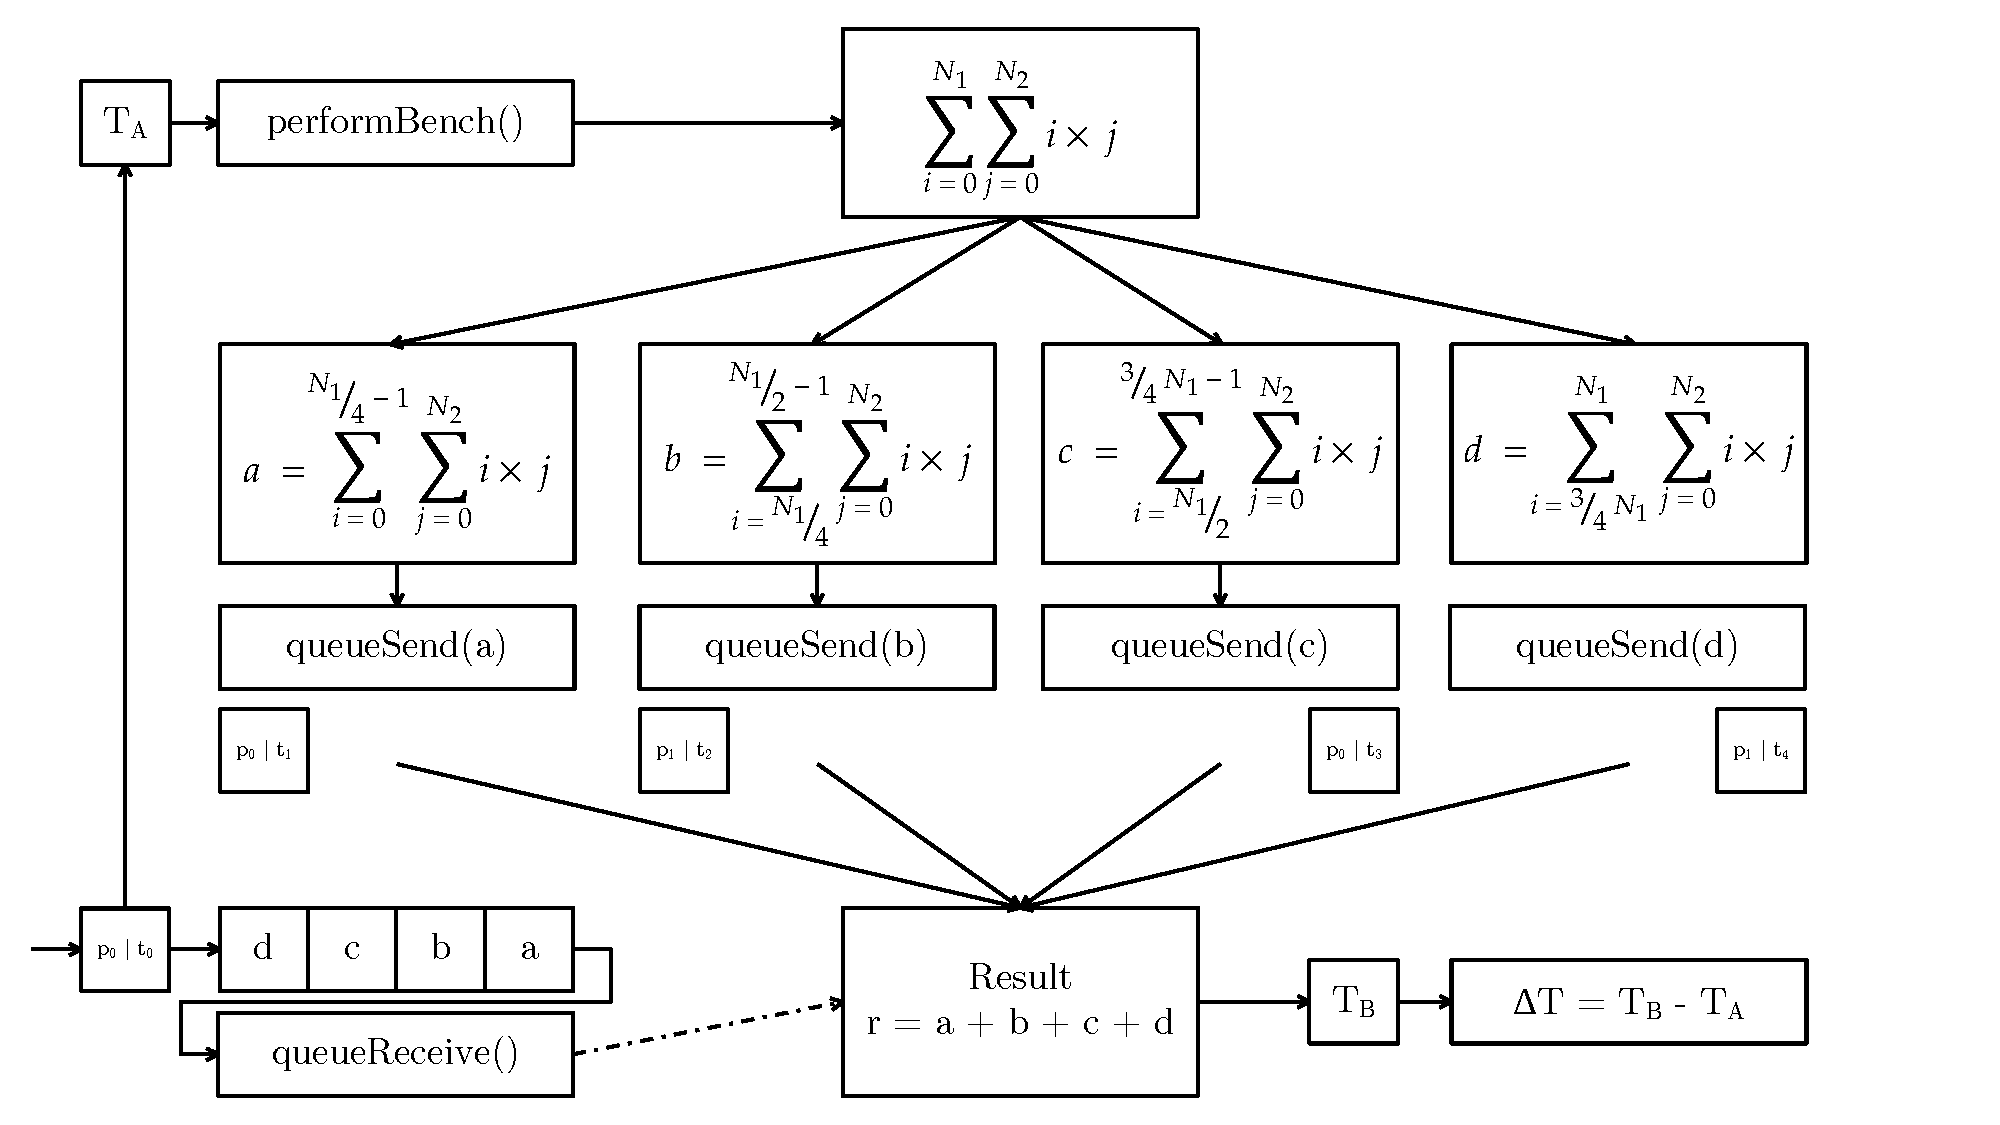
\includegraphics[width=1.1\linewidth]{images/Split-Sum-Message-Passing.pdf}}
	\caption{ Overview of the benchmark setup for the Computation example }
	\label{fig:splitSumOverview}
\end{figure}

\noindent If we now want to compare results regarding running the Computation on different cores, or even with multiple threads, we have to implement a time measurement functionality. This is done by the \textit{Benchmark.h} class. Before starting a Computation, we are saving a time stamp, and after all part results are collected, we take another one. Basically the time needed performing the tasks is the delta time between those two time stamps. But this lead into one main problem: How can we determine we collected all results, because this is an asynchronous event. 

Now our \textit{QueueHandle\_t} object will help once again. If we send back our results, the receiver will wait as long as a new object is pushed into the queue. As far as we know, we have to receive the passed \textit{numOfThreads} amount of part results. Combining these both examples will result into the following implementation:

\begin{lstlisting}[label={code:queueReceive}]
for (int k = 0; k < numOfThreads; k++) {
	long partResult;
	
	/* process communication -> receiving part results */
	xQueueReceive(*queue, &partResult, portMAX_DELAY);
	
	result += partResult;
}
\end{lstlisting}  

The last parameter for the \textit{xQueueReceive} function defines how long the receiver should wait until he should give up waiting. This is now set to a macro defining to wait as long as possible or until the queue is full. The passed reference will be used to add it to the result sum.

\newpage

\section{Introduction to the Mandelbrot fractal} \label{chap:mandelbrotIntroduction}
The Mandelbrot set is generated by iteration, which means to repeat a process over and over again. In mathematics this process is most often the application of a mathematical function.
For the Mandelbrot set, the functions involved are some of the simplest imaginable: they all are what is called quadratic polynomials and have the form f(x) = x2 + c, where c is a constant number. As we go along, we will specify exactly what value c takes.

\begin{figure}[htbp]
	\centerline{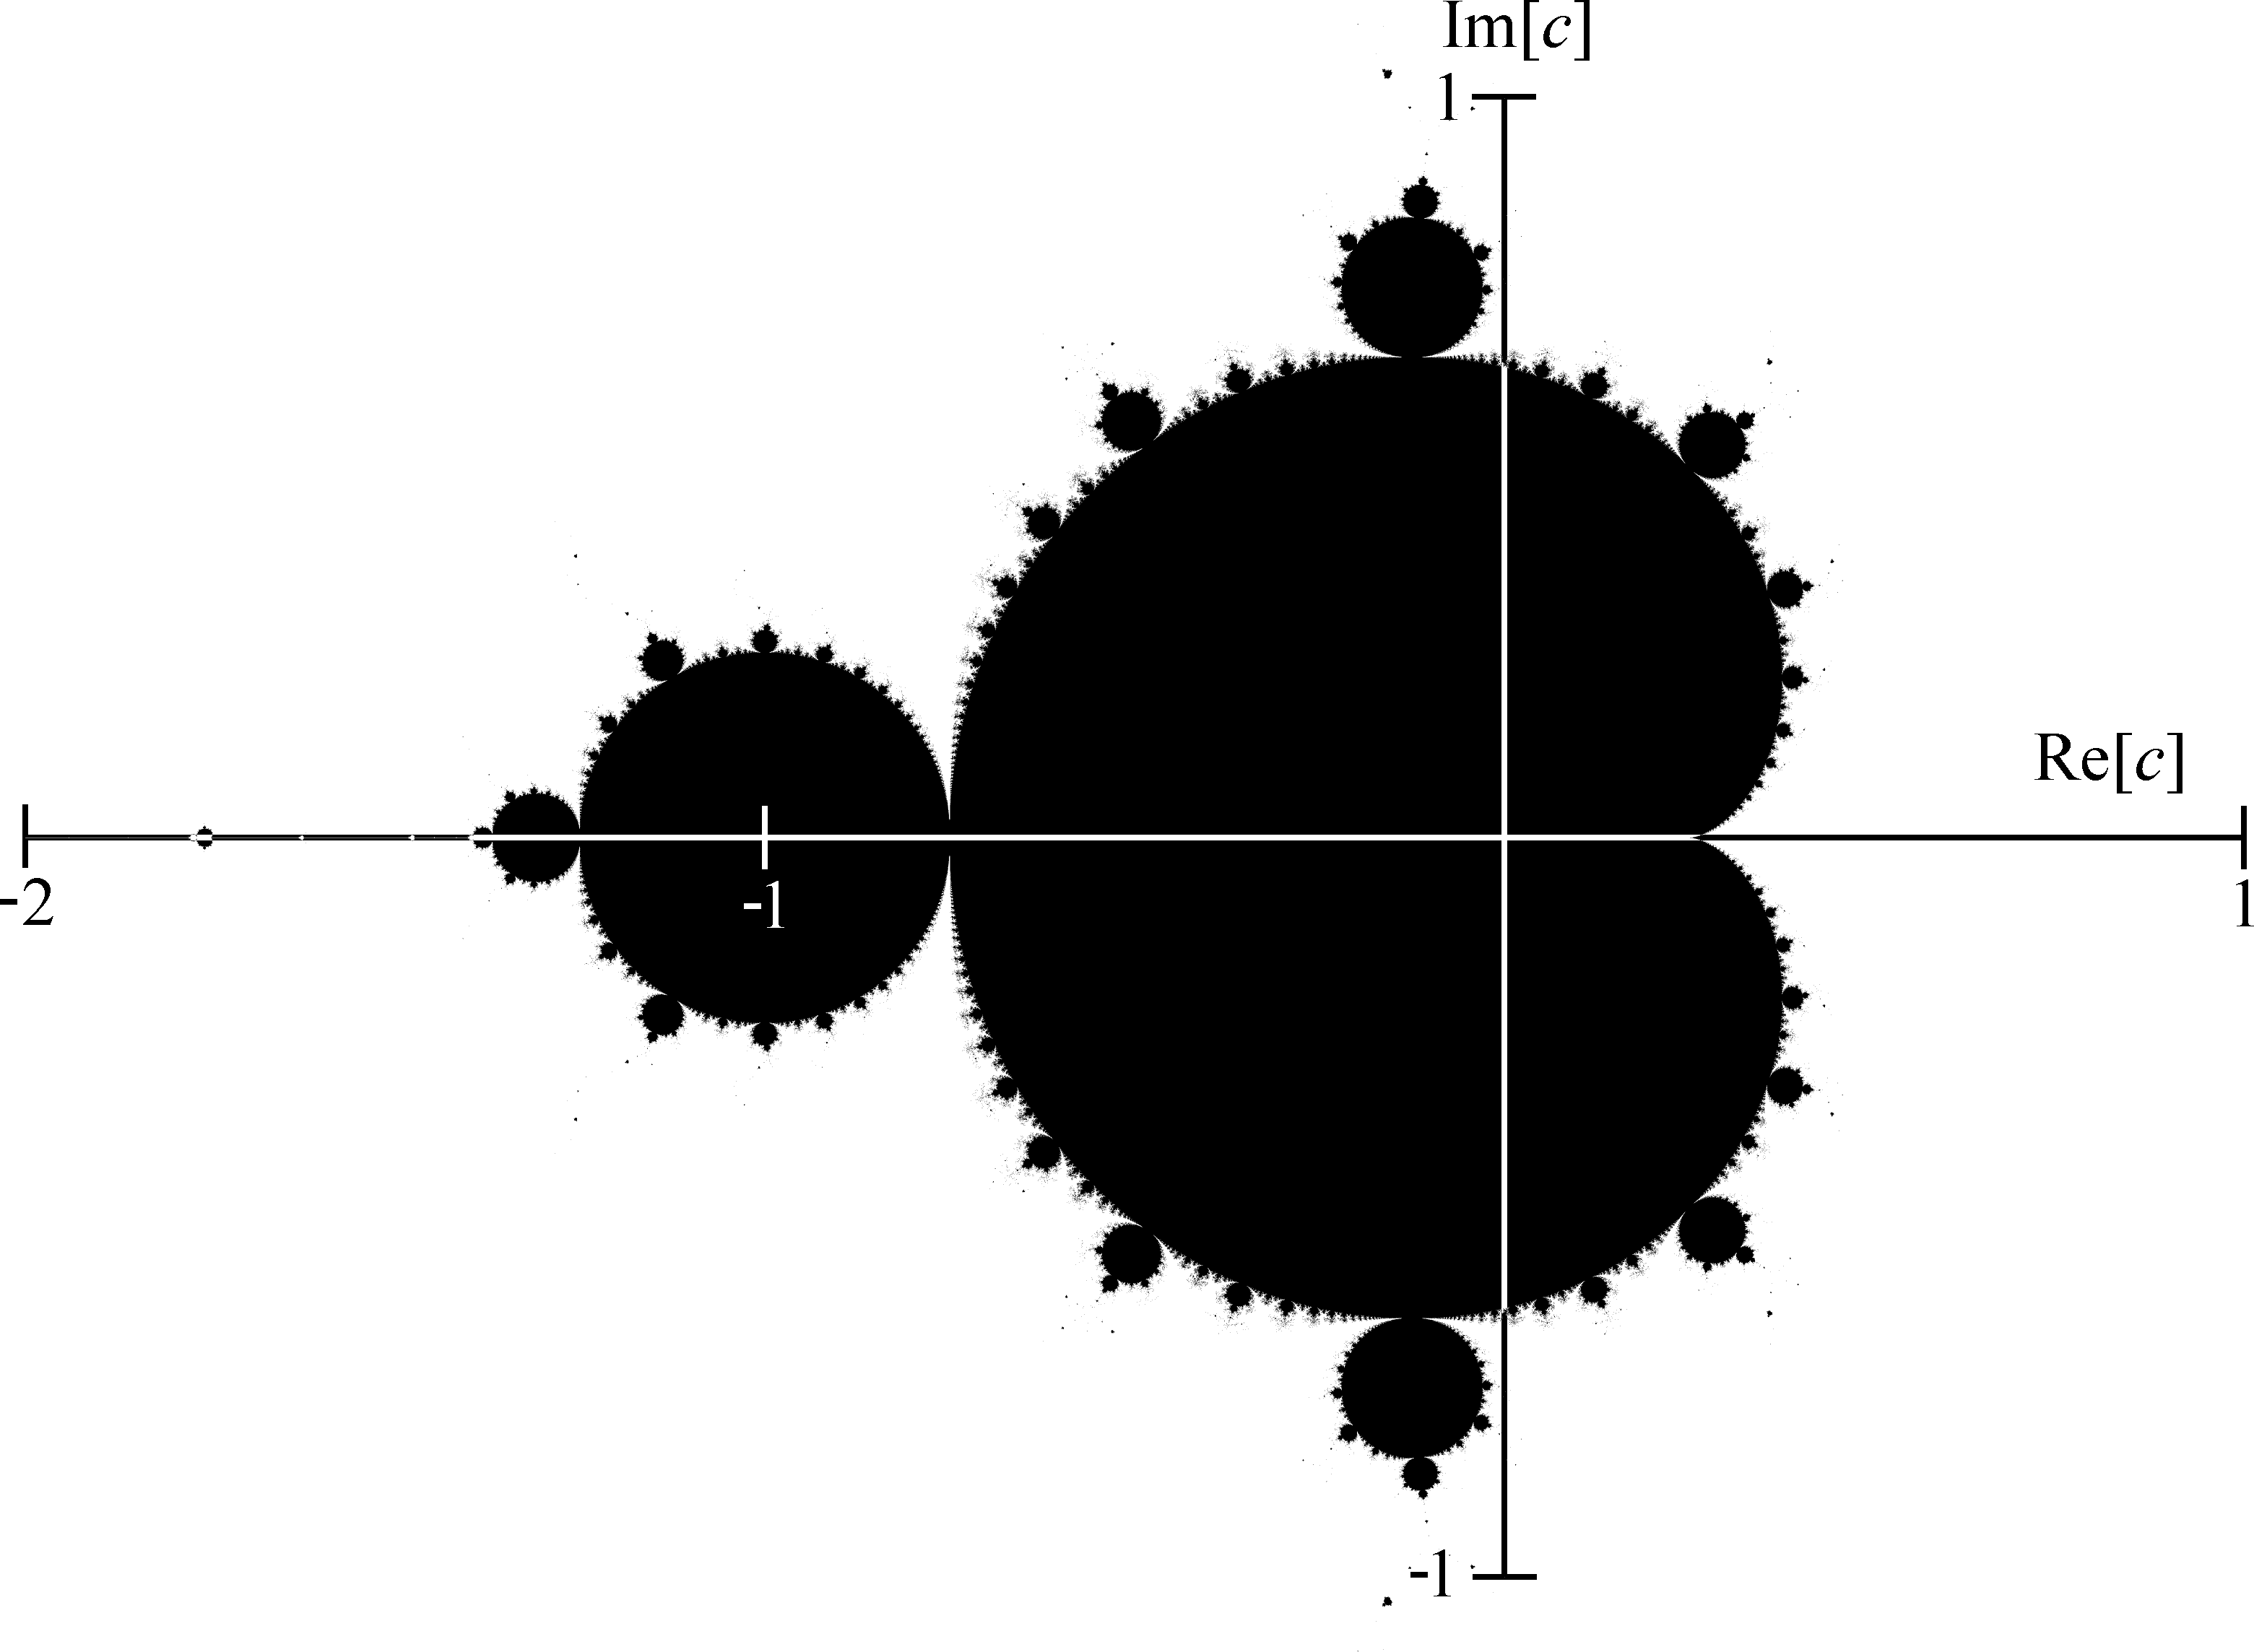
\includegraphics[width=0.9\linewidth]{images/Mandelset_hires.png}}
	\caption{ A mathematician's depiction of the Mandelbrot set M \parencite{internet14}. }
	\label{fig:mandelbrotSet}
\end{figure}  


\newpage

\section{Parallel Processing the Mandelbrot fractal}

Basically, there are no huge differences between the \textit{Benchmark} we used for the \textit{Computation} and the one we need right now for performing the Mandelbrot. What changed are the class properties and instead of a \textit{Computation.h} class we have to include the \textit{Mandelbrot.h} class. For a graphical visualization we will use instead of the uart interface a webfronted hosted on the \textit{ESP32} itself, so after the \textit{Benchmark} is done, the micro controller will create a wireless network, on which the user can log into to call the frontend in the web browser.

\subsection{Mandelbrot State Machine}

To handle all the different tasks and stages the \textit{ESP32} has to go through, we implemented a state machine.

\begin{figure}[htbp]
	\centerline{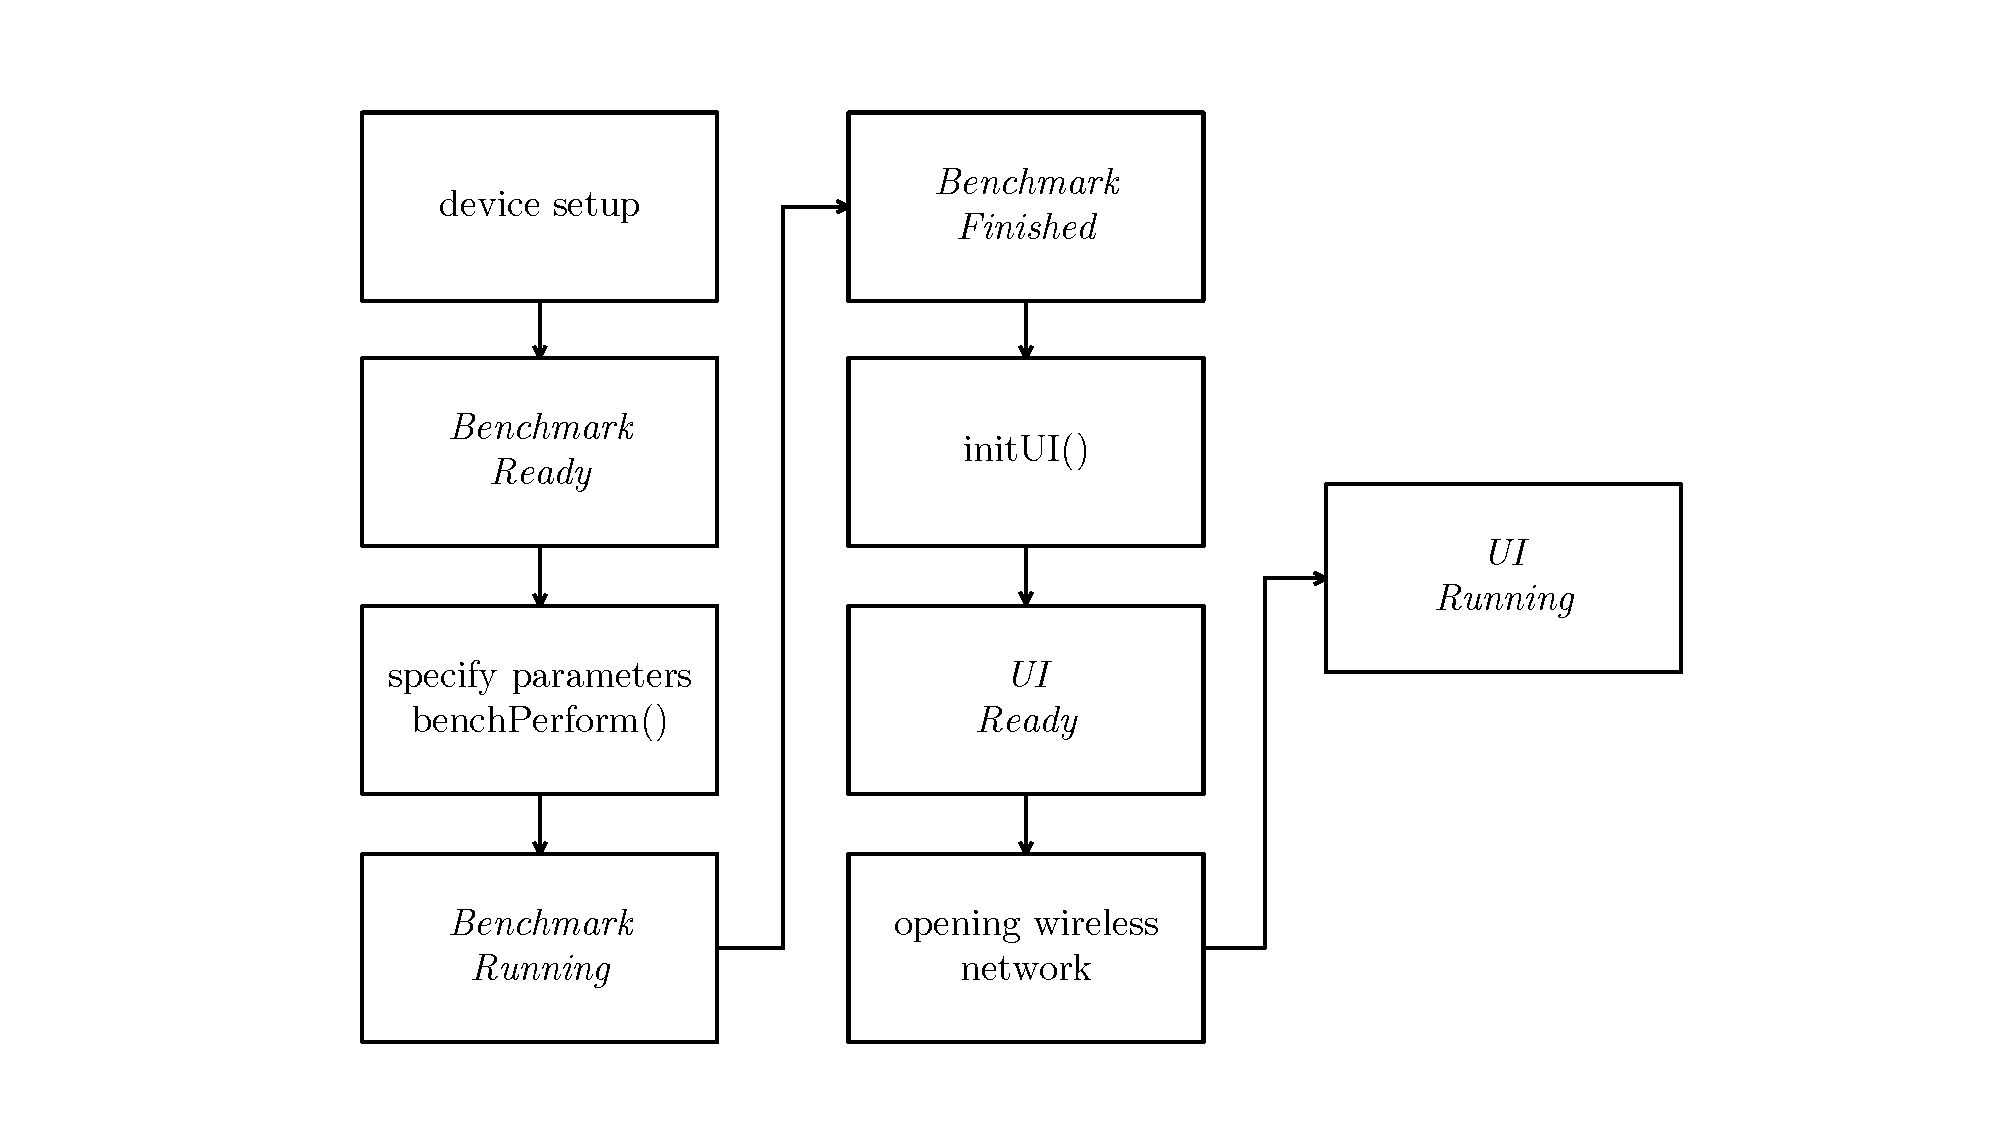
\includegraphics[width=1.1\linewidth]{images/State-Machine.pdf}}
	\caption{ State machine implementation for handling the UI, Benchmark stages }
	\label{fig:stateMachine}
\end{figure}  

Each state has its own set of parameters and will only switching the context to the next one if everything went fine. This is for preventing user errors by passing wrong arguments and to reduce runtime crashes. Nevertheless is its also necessary because the UI needs several running threads in th background as well and this would lower the overall performance of the \textit{ESP32}, which we actually need for the \text{Benchmark}.\\   

\noindent The next chapter will now focus on the details of the C++ implementation of the \textit{Benchmark} for performing the Mandelbrot computation [see Chapter \ref{subsection:backend}]. Beside that, we will describe the frontend written in \textit{javascript}, especially the communication and data processing part [see Chapter \ref{subsection:frontend}]. 

\newpage

\subsection{Mechanism to divide the picture into sub areas} \label{subsection:backend}

If now want to compute the Mandelbrot set, as we already describe in Chapter \ref{chap:mandelbrotIntroduction}, there are two possibilities to achieve this aim. And it definitely depends on the degree of complexity, which one we will choose. But first, let us describe the two main ways on how to compute the Mandelbrot set in parallel. 

Our aim is to split the image into sub sections, as we did the same for the part sums computation. What probably comes first in our mind is to split the Mandelbrot image using a division like a chess board [see Figure \ref{fig:mandelbrotChessboard}].

\begin{figure}[htbp]
	\centerline{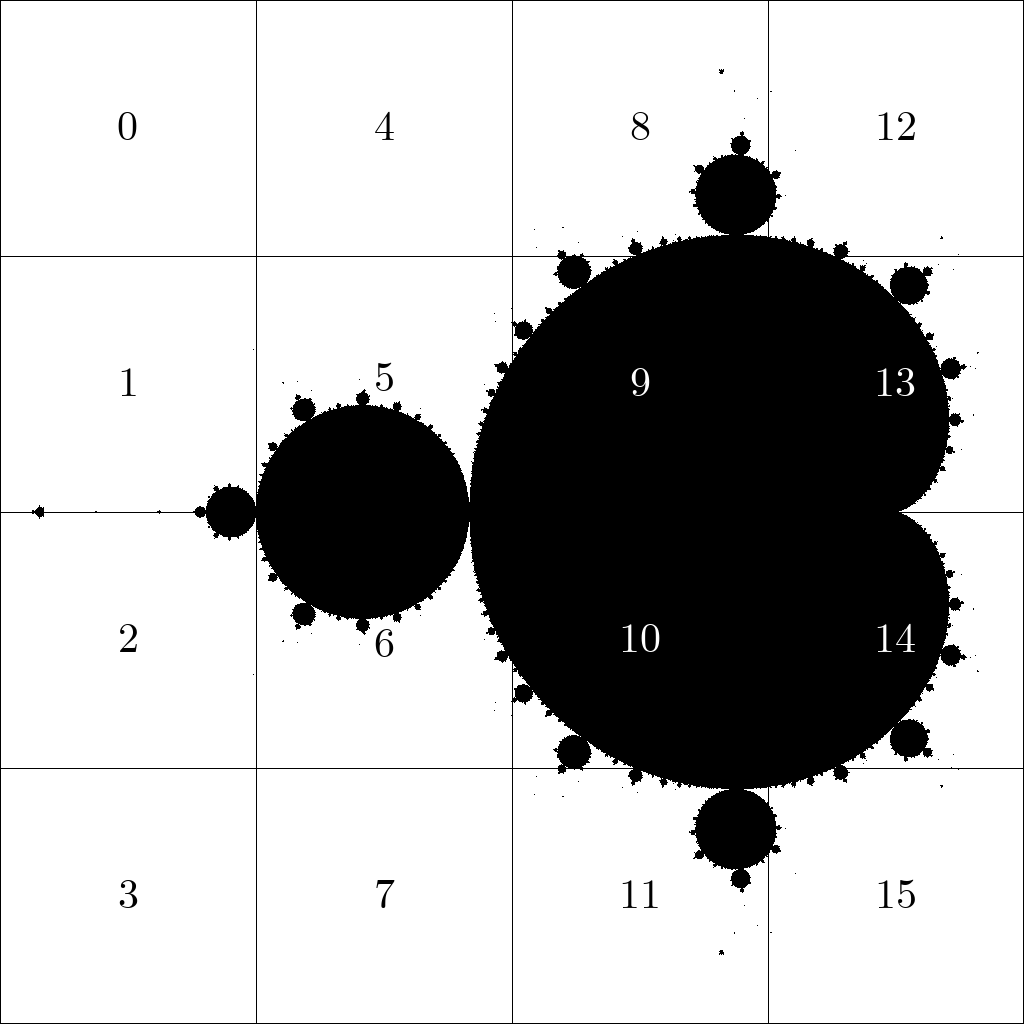
\includegraphics[width=0.75\linewidth]{images/mandelbrot-chess-board.png}}
	\caption{ Split the Mandelbrot image using the chess board method. }
	\label{fig:mandelbrotChessboard}
\end{figure} 

Each sub image is defined based on its start and end point from where its located. If we assume a resolution of 600 by 600 pixel, sub image number 5 would have its start point at P\textsubscript{5\textsubscript{Start}} (150, 150) and its end point at P\textsubscript{5\textsubscript{End}} (300, 300). Our Mandelbrot function, which has to calculate the Mandelbrot set, should receive beside the main image resolution the boundaries of the sub areas, which have to be calculated dynamically as well, so in this case the user has only to specify the number of part images, which corresponds to the number of parallel threads. The possible amount sub images are limited on two facts: for the chess board method the passed value for the number of sub images has to be a even square root and of course, the division of the width or height with the root of the passed value has to result in a even number as well.

//TODO

\newpage

\subsection{Compression for reducing file size}

...

\subsection{Graphical visualization} \label{subsection:frontend}

...\newpage

\section{Benchmark setup of the Mandelbrot fractal computation}

...
